
% !TeX program = pdflatex
\documentclass[12pt,a4paper,oneside]{article}

% PAQUETES
\usepackage[utf8]{inputenc}
\usepackage[T1]{fontenc}
\usepackage[spanish,es-tabla]{babel}
\usepackage{newtxtext,newtxmath}
\usepackage{geometry}
\usepackage{array}
\usepackage{longtable}
\usepackage{booktabs}
\usepackage{enumitem}
\usepackage{microtype}
\usepackage{setspace}
\usepackage{titlesec}
\usepackage{graphicx}
\usepackage{float}
\usepackage{caption}
\usepackage{pdflscape}
\usepackage{hyperref}

% CONFIGURACIÓN
\geometry{left=2.5cm,right=2.5cm,top=2.5cm,bottom=2.5cm}
\setstretch{1.15}
\setlength{\parindent}{1.25cm}
\setlength{\parskip}{4pt}
\renewcommand{\arraystretch}{1.25}
\setlength{\tabcolsep}{3pt}

\hypersetup{
    colorlinks=true,
    linkcolor=black,
    citecolor=black,
    urlcolor=blue,
    pdftitle={TA-IND-01 - IEEE 29148 y tipos de requisitos},
    pdfauthor={Angelina Julexy Llerena Abril}
}

\titleformat{\section}
{\normalfont\bfseries\large}{\thesection.}{0.5em}{}

\titleformat{\subsection}
{\normalfont\bfseries\normalsize}{\thesubsection.}{0.5em}{}

% COLUMNAS
\newcolumntype{C}[1]{>{\centering\arraybackslash}p{#1}}
\newcolumntype{L}[1]{>{\raggedright\arraybackslash}p{#1}}

% DATOS
\newcommand{\nombreestudiante}{Angelina Julexy Llerena Abril}
\newcommand{\paralelo}{A}
\newcommand{\fechaentrega}{07 de noviembre de 2026}
\newcommand{\sistema}{WhatsApp Web}
\newcommand{\pendiente}[1]{\textit{[Completar: #1]}}

\begin{document}

% PORTADA
\begin{titlepage}
    \centering

    {\large \textbf{UNIVERSIDAD TÉCNICA ESTATAL DE QUEVEDO}}\\[0.3cm]
    {\large Facultad de Ciencias de la Computación}\\
    {\large Carrera de Software}\\[1.5cm]

    {\Large \textbf{INGENIERÍA DE REQUERIMIENTOS}}\\[0.5cm]
    {\large ISR-401}\\[1.5cm]

    {\LARGE \textbf{TA-IND-01}}\\[0.9cm]

    \rule{0.85\textwidth}{0.5pt}\\[0.5cm]

    {\large \textbf{IEEE 29148 y tipos de requisitos de un sistema conocido}}\\
    {\large Caso de estudio: \sistema}\\[0.5cm]

    \rule{0.85\textwidth}{0.5pt}\\[2cm]

    \begin{flushleft}
        \textbf{Estudiante:} \nombreestudiante\\[0.4cm]
        \textbf{Nivel:} Cuarto\\[0.4cm]
        \textbf{Paralelo:} \paralelo\\[0.4cm]
        \textbf{Docente:} Gleiston Cicerón Guerrero Ulloa, PhD\\[0.4cm]
        \textbf{Sistema analizado:} \sistema\\[0.4cm]
        \textbf{Fecha de entrega:} \fechaentrega
    \end{flushleft}

    \vfill

    {\large Quevedo -- Ecuador}\\
    {\large 2026}

\end{titlepage}

% SISTEMA ELEGIDO
\section{Sistema elegido}

WhatsApp Web es una plataforma de mensajería instantánea que permite a los usuarios acceder a sus conversaciones desde un navegador web, sin depender exclusivamente de la aplicación móvil para comunicarse. Su propósito principal es facilitar el intercambio de mensajes y contenido multimedia, así como mantener la comunicación desde un computador. Está dirigido principalmente a personas que utilizan WhatsApp para comunicarse con familiares, amigos, compañeros de estudio y trabajo, además de usuarios que mantienen conversaciones con cuentas comerciales. Se utiliza desde computadores de escritorio o portátiles con acceso a internet, especialmente en entornos personales, académicos y laborales, donde resulta práctico escribir, consultar conversaciones y compartir archivos mientras se realizan otras actividades.


% RESUMEN ANALÍTICO
\section{Resumen analítico de ISO/IEC/IEEE 29148:2018}

\subsection{Requisito bien formado y atributos}

La cláusula 5.2.4 de la norma ISO/IEC/IEEE 29148:2018 establece que un requisito bien formado debe expresar una necesidad o capacidad que el sistema debe satisfacer de manera clara, completa y verificable. Su redacción debe permitir identificar qué se espera del sistema y bajo qué condiciones debe cumplirse, sin dejar aspectos esenciales a la interpretación del lector \cite{iso29148}.

En WhatsApp Web, un ejemplo es: «El sistema deberá permitir al usuario enviar mensajes de texto a un contacto seleccionado». El enunciado describe una capacidad concreta y puede comprobarse mediante una prueba. Esto demuestra que un requisito no debe limitarse a expresar una idea general, sino que debe comunicar una condición que pueda evaluarse.

La cláusula 5.2.8 también diferencia el requisito de sus atributos. El requisito expresa lo que el sistema debe cumplir; sus atributos aportan información para identificarlo, clasificarlo y gestionarlo. Por ejemplo, el identificador, la prioridad, la justificación, la fuente y el estado permiten administrar el requisito de envío de mensajes, pero no constituyen funciones del sistema.

\subsection{Características de un requisito individual}

De acuerdo con la cláusula 5.2.5, cada requisito debe reunir nueve características. Debe ser \textbf{necesario}, porque responde a una necesidad real; \textbf{apropiado}, porque mantiene el nivel de detalle correspondiente; y \textbf{sin ambigüedad}, porque admite una sola interpretación. Además, debe ser \textbf{completo}, al incluir la información necesaria; \textbf{singular}, al expresar una sola condición; y \textbf{factible}, porque puede cumplirse con los recursos y limitaciones existentes. También debe ser \textbf{verificable}, para comprobar objetivamente su cumplimiento; \textbf{correcto}, porque representa la necesidad de origen; y \textbf{conforme}, porque respeta la estructura y las reglas de documentación establecidas.

Estas características permiten detectar problemas antes de incorporar un requisito a la especificación. Por ejemplo, «WhatsApp Web deberá ser fácil de utilizar» no es verificable ni está libre de ambigüedad, ya que la palabra «fácil» depende de la opinión de cada usuario y no establece una medida para evaluar el resultado. La importancia de evaluar la calidad de los requisitos también ha sido abordada en investigaciones empíricas sobre este ámbito \cite{montgomery2022requirements}.


\subsection{Características de un conjunto de requisitos}

La cláusula 5.2.6 indica que un conjunto debe evaluarse como un todo. Sus requisitos deben ser \textbf{completos}, al cubrir las necesidades identificadas; \textbf{consistentes}, al no contradecirse ni duplicarse; y \textbf{factibles}, al poder realizarse dentro de las restricciones existentes. Asimismo, deben ser \textbf{comprensibles}, para que las partes interesadas entiendan lo solicitado, y el conjunto debe poder \textbf{validarse}, de modo que sea posible confirmar que responde a sus necesidades.

En WhatsApp Web, no basta con definir el envío de mensajes: también deben considerarse la recepción, el historial y el intercambio de archivos. Estos requisitos deben complementarse sin contradicciones para representar de forma coherente las capacidades esperadas del sistema. Por ello, la calidad del conjunto no depende únicamente de que cada enunciado esté bien redactado, sino también de que todos describan una solución suficiente y compatible.

\subsection{Criterios de lenguaje y términos ambiguos}

La cláusula 5.2.7 recomienda redactar los requisitos con un lenguaje preciso y evitar expresiones que permitan interpretaciones diferentes. También es importante describir qué debe lograr el sistema, sin imponer decisiones de diseño o implementación que no sean necesarias \cite{iso29148}.

Entre las expresiones que deben evitarse se encuentran los superlativos y comparativos sin parámetros, como «mejor» o «de mayor calidad»; los términos subjetivos, como «fácil» o «rentable»; y los pronombres vagos, como «esto» o «eso», cuando no tienen un referente claro. También deben evitarse adverbios y adjetivos imprecisos, como «rápidamente», «significativo» o «mínimo»; expresiones abiertas, como «pero sin limitarse a»; y condiciones indefinidas, como «si es posible» o «según corresponda». Las palabras que implican totalidad, como «siempre», «nunca» o «todo», requieren especial cuidado porque pueden establecer condiciones difíciles de demostrar. Finalmente, las referencias a otros documentos deben identificar con precisión su versión y las partes aplicables.

Por ejemplo, «WhatsApp Web deberá cargar los mensajes rápidamente» no establece un límite comprobable. En cambio, indicar un tiempo máximo y las condiciones de prueba permite medir el resultado. En conclusión, aplicar estas pautas ayuda a formular requisitos claros, verificables y coherentes, tanto de manera individual como dentro del conjunto.

% GLOSARIO
\section{Glosario de términos de la cláusula 3}

\small
\begin{longtable}{L{3.0cm} L{5.2cm} L{5.2cm}}
\caption{Glosario de términos}\label{tab:glosario}\\

\toprule
\textbf{Término} &
\textbf{Definición} &
\textbf{Ejemplo} \\
\midrule
\endfirsthead

\toprule
\textbf{Término} &
\textbf{Definición} &
\textbf{Ejemplo} \\
\midrule
\endhead

\bottomrule
\endfoot

Atributo & 
Propiedad o característica de un elemento que permite describirlo o distinguirlo mediante información cualitativa o cuantitativa. &
El requisito de enviar mensajes tiene atributos como identificador, prioridad y estado. \\

Condición &
Característica medible que establece las circunstancias o situaciones en las que debe cumplirse un requisito. &
El envío de un mensaje debe realizarse cuando el usuario tenga conexión a internet y haya seleccionado un contacto. \\

Restricción &
Limitación externa que condiciona el sistema, su diseño, implementación o desarrollo. &
WhatsApp Web requiere un navegador compatible y conexión a internet para utilizar sus funciones. \\

Contexto de uso &
Conjunto de usuarios, tareas, equipos y condiciones físicas y sociales en las que se utiliza un producto. &
Una persona utiliza WhatsApp Web desde su computadora, mediante un navegador y conexión a internet, para comunicarse mientras realiza actividades académicas. \\

Requisito derivado &
Requisito que se obtiene a partir del análisis y organización de otros requisitos dentro de una solución específica. &
A partir de la necesidad de mantener las conversaciones protegidas, se deriva el requisito de solicitar la vinculación de la cuenta antes de acceder a los mensajes. \\

Obtención de requisitos &
Proceso que utiliza técnicas organizadas para identificar y documentar las necesidades de los clientes y usuarios finales. &
Se pueden realizar entrevistas o encuestas a usuarios de WhatsApp Web para conocer sus necesidades al enviar mensajes y compartir archivos. \\

Ingeniería de requisitos &
Actividad que permite descubrir, analizar, documentar, verificar, validar y gestionar los requisitos que debe cumplir un sistema. &
Para analizar WhatsApp Web, se identifican las necesidades de los usuarios y se transforman en requisitos que posteriormente se revisan y documentan. \\

Gestión de requisitos &
Conjunto de actividades destinadas a identificar, documentar, mantener, comunicar y realizar seguimiento de los requisitos durante el ciclo de vida del sistema. &
Cuando se modifica un requisito relacionado con el envío de archivos, se actualiza su documentación y se registra el cambio correspondiente. \\

Trazabilidad de requisitos &
Identificación y documentación de las relaciones entre los requisitos y su origen o los elementos que se derivan de ellos. &
Se relaciona la necesidad de compartir archivos con el requisito que permite adjuntar y enviar documentos desde WhatsApp Web. \\

Validación de requisitos &
Confirmación de que los requisitos representan correctamente las necesidades de las partes interesadas y corresponden al sistema que se necesita. &
Se consulta a los usuarios si los requisitos definidos para enviar mensajes y compartir archivos responden a sus necesidades de comunicación. \\

\end{longtable}
\normalsize


% REQUISITOS
\section{Requisitos del sistema}

\subsection{Enunciados de los requisitos}

\begin{enumerate}[leftmargin=1.5cm]

    % Requisitos funcionales
    \item \textbf{RF-01:} El sistema deberá permitir que el usuario envíe mensajes de texto a los contactos con los que tenga una conversación activa.

    \item \textbf{RF-02:} El sistema deberá permitir que el usuario adjunte y envíe imágenes, documentos y videos desde su computador.

    \item \textbf{RF-03:} El sistema deberá mostrar el historial de mensajes de cada conversación, incluyendo el contenido y la fecha de envío.

    \item \textbf{RF-04:} El sistema deberá permitir que el usuario busque contactos y conversaciones mediante el nombre del contacto o el contenido de los mensajes.

    % Requisitos de desempeño
    \item \textbf{RD-01:} El sistema deberá mostrar los mensajes recibidos en un tiempo máximo de 2 segundos, siempre que exista una conexión a internet estable.

    \item \textbf{RD-02:} El sistema deberá cargar una conversación con hasta 1000 mensajes en un tiempo máximo de 3 segundos, bajo condiciones normales de conexión y funcionamiento.

    % Requisito de interfaz externa
    \item \textbf{RI-01:} El sistema deberá permitir la vinculación de la cuenta de WhatsApp mediante el escaneo de un código QR utilizando la aplicación móvil.

    % Requisito de proceso
    \item \textbf{RP-01:} El proceso de envío de un mensaje deberá registrar su estado como pendiente, enviado, entregado o leído, según la información disponible del sistema.

    % Requisitos de calidad
    \item \textbf{RQ-01:} El sistema deberá mantener una disponibilidad mínima del 99\% durante cada mes de funcionamiento.

    \item \textbf{RQ-02:} El sistema deberá garantizar que el contenido de los mensajes solo sea accesible para los participantes autorizados de la conversación.

    \item \textbf{RQ-03:} El sistema deberá mantener la compatibilidad con las dos versiones más recientes de los navegadores Google Chrome, Mozilla Firefox y Microsoft Edge.

    \item \textbf{RQ-04:} El sistema deberá conservar la integridad de los archivos enviados, de manera que el archivo recibido coincida con el archivo original.

    \item \textbf{RQ-05:} El sistema deberá recuperar el acceso a las conversaciones en un tiempo máximo de 30 segundos después de restablecerse una interrupción de la conexión a internet.

    % Requisitos de usabilidad o calidad en uso
    \item \textbf{RU-01:} Al menos el 90\% de los usuarios participantes deberá completar el envío de un mensaje de texto sin asistencia durante una prueba de usabilidad.

    \item \textbf{RU-02:} Al menos el 90\% de los usuarios participantes deberá localizar una conversación específica en un tiempo máximo de 30 segundos durante una prueba de usabilidad.

\end{enumerate}


%
% CLASIFICACIÓN
\section{Clasificación de los requisitos}

Los requisitos de calidad del producto se relacionan con el modelo ISO/IEC 25010:2023, mientras que los requisitos de calidad en uso se clasifican mediante el modelo ISO/IEC 25019:2023 \cite{iso25010,iso25019}.

\small
\begin{longtable}{C{1.1cm} L{4.0cm} L{2.0cm} L{3.0cm} L{4.0cm}}

\caption{Clasificación de los requisitos}\label{tab:clasificacion}\\

\toprule
\textbf{ID} &
\textbf{Enunciado} &
\textbf{Tipo} &
\textbf{Característica ISO/IEC 25010} &
\textbf{Métrica y criterio de aceptación} \\

\midrule
\endfirsthead

\toprule
\textbf{ID} &
\textbf{Enunciado} &
\textbf{Tipo} &
\textbf{Característica ISO/IEC 25010} &
\textbf{Métrica y criterio de aceptación} \\

\midrule
\endhead

\bottomrule
\endfoot

RF-01 &
El sistema deberá permitir que el usuario envíe mensajes de texto a los contactos con los que tenga una conversación activa. &
Funcional &
No aplica &
Porcentaje de mensajes enviados correctamente. Se acepta si el 100\% de los mensajes de prueba se envía al contacto seleccionado. \\

RF-02 &
El sistema deberá permitir que el usuario adjunte y envíe imágenes, documentos y videos desde su computador. &
Funcional &
No aplica &
Porcentaje de archivos adjuntados y enviados correctamente. Se acepta si el 100\% de los archivos de prueba se envía sin errores. \\

RF-03 &
El sistema deberá mostrar el historial de mensajes de cada conversación, incluyendo el contenido y la fecha de envío. &
Funcional &
No aplica &
Porcentaje de mensajes del historial mostrados correctamente. Se acepta si el 100\% de los mensajes de prueba presenta su contenido y fecha de envío. \\

RF-04 &
El sistema deberá permitir que el usuario busque contactos y conversaciones mediante el nombre del contacto o el contenido de los mensajes. &
Funcional &
No aplica &
Porcentaje de búsquedas que devuelven resultados correspondientes. Se acepta si el 100\% de las búsquedas de prueba muestra los resultados esperados. \\

RD-01 &
El sistema deberá mostrar los mensajes recibidos en un tiempo máximo de 2 segundos, siempre que exista una conexión a internet estable. &
Desempeño &
Eficiencia de desempeño -- Comportamiento temporal &
Tiempo de respuesta. Se acepta si los mensajes recibidos se muestran en un máximo de 2 segundos durante las pruebas. \\

RD-02 &
El sistema deberá cargar una conversación con hasta 1000 mensajes en un tiempo máximo de 3 segundos, bajo condiciones normales de conexión y funcionamiento. &
Desempeño &
Eficiencia de desempeño -- Comportamiento temporal &
Tiempo de carga. Se acepta si una conversación de hasta 1000 mensajes se carga en un máximo de 3 segundos durante las pruebas. \\

RI-01 &
El sistema deberá permitir la vinculación de la cuenta de WhatsApp mediante el escaneo de un código QR utilizando la aplicación móvil. &
Interfaz externa &
Compatibilidad -- Interoperabilidad &
Porcentaje de vinculaciones exitosas. Se acepta si el 100\% de los intentos de prueba permite vincular la cuenta mediante el código QR. \\

RP-01 &
El proceso de envío de un mensaje deberá registrar su estado como pendiente, enviado, entregado o leído, según la información disponible del sistema. &
Proceso &
No aplica &
Porcentaje de cambios de estado registrados correctamente. Se acepta si el 100\% de las transiciones de estado de los mensajes de prueba se registra de acuerdo con el resultado del envío. \\

RQ-01 &
El sistema deberá mantener una disponibilidad mínima del 99\% durante cada mes de funcionamiento. &
Calidad &
Fiabilidad -- Disponibilidad &
Porcentaje de disponibilidad mensual. Se acepta si el sistema permanece operativo al menos el 99\% del tiempo mensual evaluado. \\

RQ-02 &
El sistema deberá garantizar que el contenido de los mensajes solo sea accesible para los participantes autorizados de la conversación. &
Calidad &
Seguridad -- Confidencialidad &
Porcentaje de intentos de acceso no autorizado en los que el contenido permanece inaccesible. Se acepta si el 100\% de los intentos de prueba impide consultar el contenido de los mensajes. \\

RQ-03 &
El sistema deberá mantener la compatibilidad con las dos versiones más recientes de los navegadores Google Chrome, Mozilla Firefox y Microsoft Edge. &
Calidad &
Flexibilidad -- Adaptabilidad &
Número de versiones de navegadores compatibles. Se acepta si el sistema funciona correctamente en las dos versiones más recientes de cada uno de los tres navegadores indicados. \\

RQ-04 &
El sistema deberá conservar la integridad de los archivos enviados, de manera que el archivo recibido coincida con el archivo original. &
Calidad &
Seguridad -- Integridad &
Porcentaje de archivos recibidos sin alteraciones. Se acepta si el 100\% de los archivos de prueba coincide con el archivo original. \\

RQ-05 &
El sistema deberá recuperar el acceso a las conversaciones en un tiempo máximo de 30 segundos después de restablecerse una interrupción de la conexión a internet. &
Calidad &
Fiabilidad -- Capacidad de recuperación &
Tiempo de recuperación. Se acepta si el acceso a las conversaciones se restablece en un máximo de 30 segundos después de recuperar la conexión. \\

RU-01 &
Al menos el 90\% de los usuarios participantes deberá completar el envío de un mensaje de texto sin asistencia durante una prueba de usabilidad. &
Calidad en uso &
Efectividad -- ISO/IEC 25019:2023 &
Porcentaje de usuarios que completan la tarea sin asistencia. Se acepta si al menos el 90\% de los participantes envía un mensaje sin ayuda. \\

RU-02 &
Al menos el 90\% de los usuarios participantes deberá localizar una conversación específica en un tiempo máximo de 30 segundos durante una prueba de usabilidad. &
Calidad en uso &
Eficiencia -- ISO/IEC 25019:2023 &
Porcentaje de usuarios que localizan la conversación en 30 segundos o menos. Se acepta si al menos el 90\% de los participantes completa la tarea dentro del tiempo establecido. \\

\end{longtable}
\normalsize


% AUTOEVALUACIÓN
\section{Autoevaluación y corrección de los requisitos}

\small
\begin{longtable}{C{1.3cm} L{4.0cm} L{3.6cm} L{4.2cm}}

\caption{Autoevaluación de los requisitos}\label{tab:auto}\\

\toprule
\textbf{ID} &
\textbf{Versión anterior} &
\textbf{Propiedad incumplida} &
\textbf{Versión corregida} \\

\midrule
\endfirsthead

\toprule
\textbf{ID} &
\textbf{Versión anterior} &
\textbf{Propiedad incumplida} &
\textbf{Versión corregida} \\

\midrule
\endhead

\bottomrule
\endfoot

RF-01 &
El sistema deberá permitir enviar mensajes fácilmente. &
Sin ambigüedad y verificable: el término ``fácilmente'' es subjetivo y no permite comprobar el cumplimiento. &
El sistema deberá permitir que el usuario envíe mensajes de texto a los contactos con los que tenga una conversación activa. \\

RF-02 &
El sistema deberá permitir enviar archivos y otros contenidos. &
Completo y sin ambigüedad: no especifica los tipos de archivos ni desde dónde se adjuntan. &
El sistema deberá permitir que el usuario adjunte y envíe imágenes, documentos y videos desde su computador. \\

RF-03 &
El sistema deberá mostrar los mensajes anteriores. &
Completo y verificable: no indica qué información debe mostrar cada mensaje. &
El sistema deberá mostrar el historial de mensajes de cada conversación, incluyendo el contenido y la fecha de envío. \\

RF-04 &
El sistema deberá permitir buscar cualquier cosa dentro de WhatsApp. &
Apropiado y sin ambigüedad: la expresión ``cualquier cosa'' no delimita los elementos que se pueden buscar. &
El sistema deberá permitir que el usuario busque contactos y conversaciones mediante el nombre del contacto o el contenido de los mensajes. \\

RD-01 &
Los mensajes deberán aparecer rápidamente. &
Verificable y sin ambigüedad: ``rápidamente'' no establece un límite de tiempo medible. &
El sistema deberá mostrar los mensajes recibidos en un tiempo máximo de 2 segundos, siempre que exista una conexión a internet estable. \\

RD-02 &
Las conversaciones deberán cargar en poco tiempo. &
Verificable y completo: no establece el tiempo máximo ni la cantidad de mensajes considerada. &
El sistema deberá cargar una conversación con hasta 1000 mensajes en un tiempo máximo de 3 segundos, bajo condiciones normales de conexión y funcionamiento. \\

RI-01 &
El usuario deberá conectarse mediante un código de forma sencilla. &
Sin ambigüedad y verificable: no identifica el código ni el mecanismo externo utilizado. &
El sistema deberá permitir la vinculación de la cuenta de WhatsApp mediante el escaneo de un código QR utilizando la aplicación móvil. \\

RP-01 &
El sistema deberá mostrar correctamente el estado de los mensajes. &
Completo y verificable: no especifica los estados que deben registrarse. &
El proceso de envío de un mensaje deberá registrar su estado como pendiente, enviado, entregado o leído, según la información disponible del sistema. \\

RQ-01 &
El sistema deberá estar disponible siempre. &
Factible y verificable: ``siempre'' establece una condición absoluta sin un umbral medible. &
El sistema deberá mantener una disponibilidad mínima del 99\% durante cada mes de funcionamiento. \\

RQ-02 &
El sistema deberá proteger muy bien los mensajes. &
Sin ambigüedad y verificable: ``muy bien'' no define la protección requerida ni cómo comprobarla. &
El sistema deberá garantizar que el contenido de los mensajes solo sea accesible para los participantes autorizados de la conversación. \\

RQ-03 &
El sistema deberá funcionar en todos los navegadores. &
Factible y verificable: ``todos'' no delimita los navegadores ni sus versiones. &
El sistema deberá mantener la compatibilidad con las dos versiones más recientes de los navegadores Google Chrome, Mozilla Firefox y Microsoft Edge. \\

RQ-04 &
Los archivos deberán llegar correctamente. &
Sin ambigüedad y verificable: ``correctamente'' no define qué condición deben cumplir los archivos recibidos. &
El sistema deberá conservar la integridad de los archivos enviados, de manera que el archivo recibido coincida con el archivo original. \\

RQ-05 &
El sistema deberá recuperar la conexión lo más rápido posible. &
Verificable y sin ambigüedad: ``lo más rápido posible'' no establece un tiempo máximo de recuperación. &
El sistema deberá recuperar el acceso a las conversaciones en un tiempo máximo de 30 segundos después de restablecerse una interrupción de la conexión a internet. \\

RU-01 &
Los usuarios deberán poder enviar mensajes sin dificultad. &
Verificable y sin ambigüedad: no establece cómo se medirá la facilidad de uso ni el resultado esperado. &
Al menos el 90\% de los usuarios participantes deberá completar el envío de un mensaje de texto sin asistencia durante una prueba de usabilidad. \\

RU-02 &
Los usuarios deberán encontrar sus conversaciones rápidamente. &
Verificable y sin ambigüedad: ``rápidamente'' no establece un tiempo límite ni un porcentaje de cumplimiento. &
Al menos el 90\% de los usuarios participantes deberá localizar una conversación específica en un tiempo máximo de 30 segundos durante una prueba de usabilidad. \\

\end{longtable}
\normalsize


% REFLEXIÓN
\section{Reflexión}

Para esta reflexión, considero que los requisitos de calidad fueron los que presentaron mayor dificultad, principalmente porque no basta con describir cómo debería comportarse el sistema, sino que también es necesario identificar una característica y subcaracterística de la norma ISO/IEC 25010:2023 que se relacione correctamente con cada requisito. Además, fue necesario establecer métricas y criterios de aceptación que permitieran comprobar su cumplimiento, utilizando valores específicos en lugar de expresiones subjetivas como «rápidamente» o «correctamente».

En el caso de WhatsApp Web, algunos aspectos, como la disponibilidad, la seguridad y la recuperación ante interrupciones de conexión, requirieron analizar qué condiciones podían medirse y cómo establecer un límite para evaluarlas. También fue importante diferenciar los requisitos de calidad del producto de los requisitos de calidad en uso, ya que estos últimos se relacionan con los resultados que obtienen los usuarios al utilizar el sistema.

Esta actividad me permitió comprender que redactar requisitos no consiste únicamente en describir las funciones de un sistema, sino en expresar sus necesidades de manera clara, precisa y verificable. También entendí la importancia de revisar cada enunciado para evitar ambigüedades y asegurar que pueda ser evaluado durante el desarrollo y las pruebas del software.

% EVIDENCIAS
\section{Evidencias}

\begin{figure}[H]
    \centering
    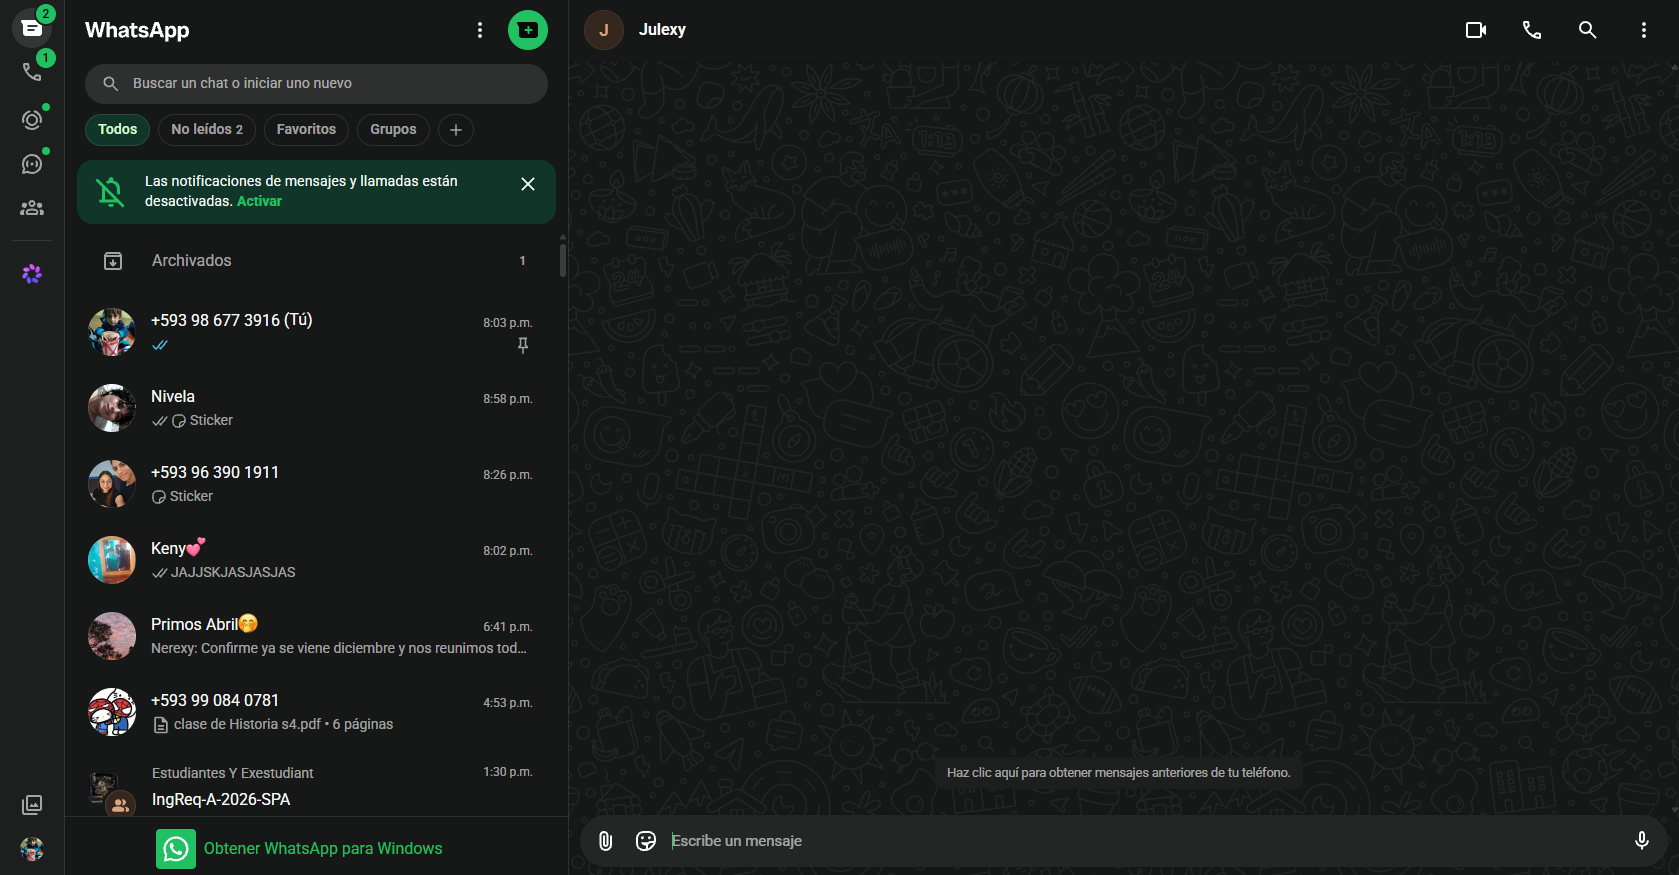
\includegraphics[width=0.90\textwidth]{figuras/whatsapp_mensajes.png}
    \caption{Interfaz de conversaciones de WhatsApp Web.}
    \label{fig:mensajes}
\end{figure}

\begin{figure}[H]
    \centering
    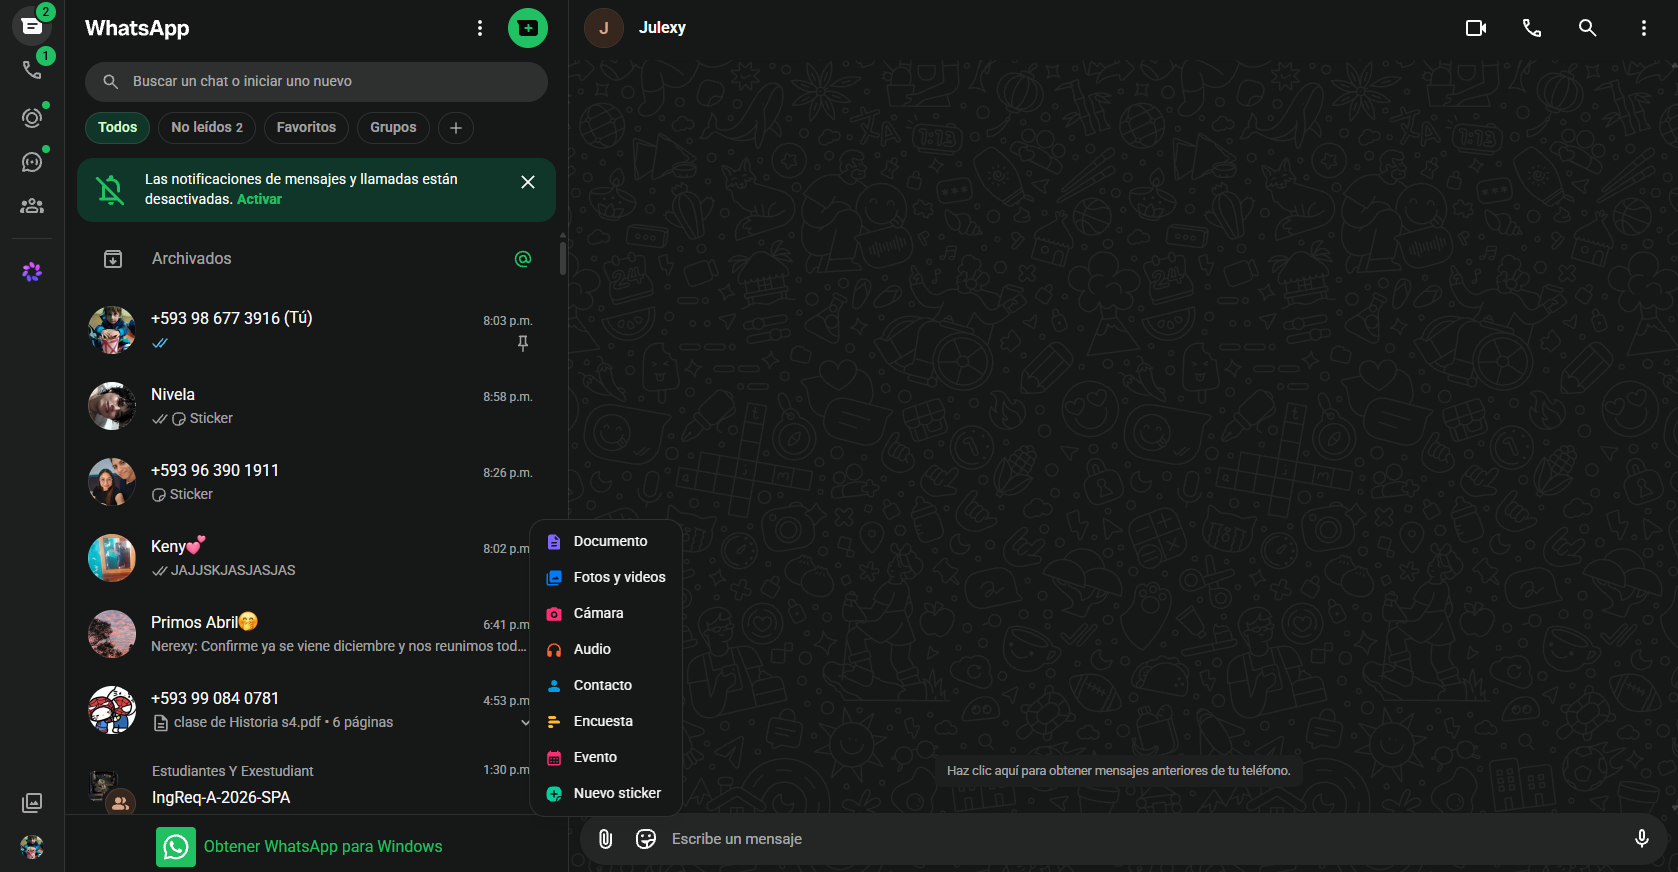
\includegraphics[width=0.90\textwidth]{figuras/whatsapp_archivos.png}
    \caption{Opciones para adjuntar y compartir archivos.}
    \label{fig:archivos}
\end{figure}

\begin{figure}[H]
    \centering
    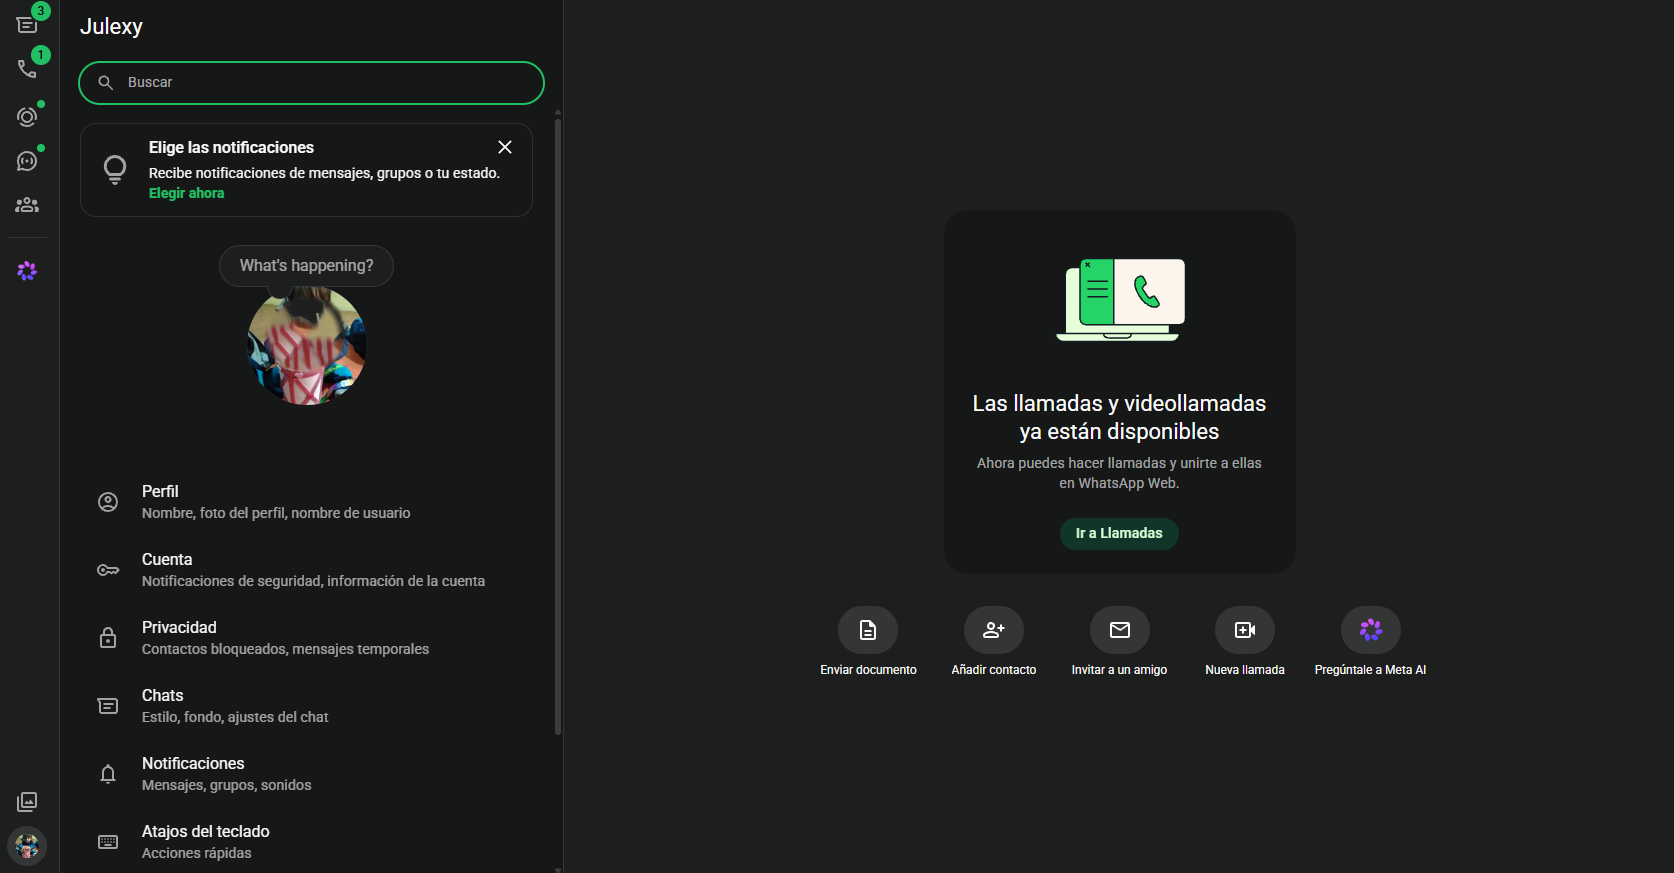
\includegraphics[width=0.90\textwidth]{figuras/whatsapp_perfil.png}
    \caption{Opciones de perfil o configuración de WhatsApp Web.}
    \label{fig:perfil}
\end{figure}

% DECLARACIÓN
\section{Declaración de uso de herramientas de apoyo}

Para realizar esta actividad, se utilizaron Claude Sonnet 5.5, de Anthropic, y ChatGPT GPT-6, de OpenAI, como herramientas de apoyo para revisar la redacción, identificar ambigüedades y solucionar errores relacionados con el código LaTeX. También se emplearon para verificar que los requisitos estuvieran clasificados correctamente. Cuando se identificaron errores, se solicitó su corrección y la respectiva justificación. Las recomendaciones proporcionadas fueron analizadas y consideradas para realizar los ajustes necesarios en el documento.

% REFERENCIAS
\bibliographystyle{IEEEtran}
\bibliography{referencias}

\end{document}